\documentclass[12pt]{report}
\setlength{\textwidth}{6.5 in}
\setlength{\evensidemargin}{0 in}
\setlength{\oddsidemargin}{0 in}
\setlength{\textheight}{9.4 in }
\setlength{\topmargin}{-0.7 in}
\pagestyle{myheadings}
\markboth{\em EE264: Homework \#05}{\em EE264: Homework \#05}
\usepackage[pdftex]{graphicx} \usepackage{eso-pic}
\usepackage{amsmath}
\usepackage{amssymb}
\usepackage{graphicx}
\usepackage{ifthen}
\usepackage{tikz}
\usepackage{pgfplots}
\usepackage{array}  % for table column M
\usepackage{makecell} % to break line within a cell
\usepackage{verbatim}
\usepackage{epstopdf}
\usepackage{amsfonts}
\usepackage{xcolor}
\usepackage{subcaption}
\usepackage{pdfpages}
\usepackage{hyperref}
%\captionsetup{compatibility=false}
%\usepackage{dsfont}
\usepackage{placeins}
\usepackage[absolute,overlay]{textpos}
\usetikzlibrary{calc, angles,quotes}
\usetikzlibrary{pgfplots.fillbetween, backgrounds}
\usetikzlibrary{positioning}
\usetikzlibrary{arrows}
\usetikzlibrary{pgfplots.groupplots}
\usetikzlibrary{arrows.meta}
\usetikzlibrary{plotmarks}
\usetikzlibrary{decorations.markings}

\DeclareGraphicsExtensions{.pdf,.eps,.png}

\def\thickness{very thick}

\tikzset{
amark/.style 2 args={
	decoration={             
		markings, 
		mark=at position {0.5} with { 
			\arrow{stealth},
			\node[#2] {#1};
		}
	}, \thickness,
	postaction={decorate}
},
earlymark/.style 2 args={
	decoration={             
		markings, 
		mark=at position {0.25} with { 
			\arrow{stealth},
			\node[#2] {#1};
		}
	}, \thickness,
	postaction={decorate}
},
latemark/.style 2 args={
	decoration={             
		markings, 
		mark=at position {0.8} with { 
			\arrow{stealth},
			\node[#2] {#1};
		}
	}, \thickness,
	postaction={decorate}
},
zpath/.style={
	decoration={             
		markings, 
		mark=at position {0.5} with { 
			\arrow{stealth},
			\node[#1] {$z^{-1}$};
		}
	}, \thickness,
	postaction={decorate}
},
terminal/.style 2 args={draw,circle,inner sep=2pt,label={#1:#2}},
}

\definecolor{matlabcomment}{RGB}{34,139,34}

\pgfmathdeclarefunction{gauss}{1}{%
	\pgfmathparse{1/(sqrt(2*pi))*exp(-((#1)^2)/2)}%
}

\pgfmathdeclarefunction{laplacian}{2}{%
	\pgfmathparse{1/(#2*2)*exp(-(abs(x-#1))/(#2))}%
}

\pgfmathdeclarefunction{pretty_func}{1}{%
	\pgfmathparse{cos(deg(#1/2)) - sin(deg(#1)) + cos(deg(#1/2)-45) - sin(deg(#1/4)-154)}%
}

\pgfplotsset{
	dirac/.style={
		mark=triangle*,
		mark options={scale=2},
		ycomb,
		scatter,
		visualization depends on={y/abs(y)-1 \as \sign},
		scatter/@pre marker code/.code={\scope[rotate=90*\sign,yshift=-2pt]}
	}
}

\def\thickness{very thick}

\tikzset{
amark/.style 2 args={
	decoration={             
		markings, 
		mark=at position {0.5} with { 
			\arrow{stealth},
			\node[#2] {#1};
		}
	}, \thickness,
	postaction={decorate}
},
earlymark/.style 2 args={
	decoration={             
		markings, 
		mark=at position {0.25} with { 
			\arrow{stealth},
			\node[#2] {#1};
		}
	}, \thickness,
	postaction={decorate}
},
latemark/.style 2 args={
	decoration={             
		markings, 
		mark=at position {0.8} with { 
			\arrow{stealth},
			\node[#2] {#1};
		}
	}, \thickness,
	postaction={decorate}
},
zpath/.style={
	decoration={             
		markings, 
		mark=at position {0.5} with { 
			\arrow{stealth},
			\node[#1] {$z^{-1}$};
		}
	}, \thickness,
	postaction={decorate}
},
terminal/.style 2 args={draw,circle,inner sep=2pt,label={#1:#2}},
}


\tikzset{
	invisible/.style={opacity=0},
	visible on/.style={alt={#1{}{invisible}}},
	alt/.code args={<#1>#2#3}{%
		\alt<#1>{\pgfkeysalso{#2}}{\pgfkeysalso{#3}} % \pgfkeysalso doesn't change the path
	},
}

\newcommand\PlotSampledSpectrum[4]{%
	\def\fs{#2}%
	\def\fmax{#3}%
	\def\ros{#4}%
	\input{#1}%
}

\pgfmathdeclarefunction{invgauss}{2}{%
	\pgfmathparse{sqrt(-2*ln(#1))*cos(deg(2*pi*#2))}%
}

\tikzset{
	declare function={
		sinc(\x) = (and(\x!=0, 1) * (sin(deg(pi*\x))/(pi*\x)) +
		(and(\x==0, 1) * 1);
	}
}

\DeclareMathOperator{\E}{\mathbb{E}} % expectation

\newcommand\SimpleSys[4]{%
	\def\xin{#2}%
	\def\Hz{#3}%
	\def\yout{#4}
	\input{#1}%
}

\begin{document}
\thispagestyle{empty}
\begin{centering}
	{\large Stanford University}\\
	{\large EE 264: Digital Signal Processing}\\
	{\large Summer, 2018} \\
	\mbox{}\\
	{\large Homework \#05}\\
	\mbox{}\\
\end{centering}
\noindent Date assigned:  July 28, 2018 \hfill
Date due: August 5, 2018\\
\noindent \rule{6.5 in}{0.5pt}
%\mbox{}\\
\noindent {\bf Reading:}  This assignment covers primarily lecture 8 - July 30 (Problem 1-2) and lecture 9 - August 1 (Problem 3-6). \\
\noindent {\bf Homework submission:}  Please submit your solutions on Gradescope. Create a single .pdf file containing all your analytical derivations, sketches, plots, and Matlab code (if any). \\
\noindent
\rule{6.5 in}{0.5pt}
\mbox{}\\

\noindent {\bf Problem 1: (25 points)}

Consider the system of Example 5.8 of the textbook. Its system function is
\begin{equation}
H(z) = 0.05634\frac{(1+z^{-1})(1 -1.0166z^{-1} + z^{-2})}{(1-0.683z^{-1})(1 -1.4461z^{-1} + 0.7957z^{-2})}
\end{equation}

\begin{description}
	\item[(a)] Draw the signal flow graph of an implementation of the system as a cascade of a second-order system with a first-order system. Mark the values of the coefficients on the signal flow graph.
	\item[(b)] Draw a direct form II signal flow graph for implementing the system as a single third-order flow graph. 
	\item[(c)] Plot the pole-zero diagram of $H(z)$ for the unquantified coefficients. You may use \texttt{conv} to multiply out the numerator and denominator and obtain the coefficients vectors \texttt{a} and \texttt{b}. Then use \texttt{zplane} to plot the pole-zero diagram.
	\item[(d)] Quantize the filter coefficients with 6 bits to the right of the imagined binary point. Call the Q6-quantized coefficient vectors \texttt{ah} and \texttt{bh}. Then compare the pole-zero locations using
	\begin{align*}
		&\texttt{plot(roots(b),`ok');~plot(roots(a),`xk'); hold on} \\
		&\texttt{plot(roots(bh),`or');~plot(roots(ah),`xr');}
	\end{align*}
	
	Also plot the log magnitude of the frequency response of both the ``unquantized" and Q6-quantized coefficients on the same graph. Hand in both plots. You should observe that there is very little difference between the quantized and unquantized systems. What is your intuition about why this is so?
	
\end{description}

\mbox{}\\
\newpage
\noindent {\bf Problem 2: (25 points)} (from the midterm of Spring-2014)

The following flow graphs represent equivalent difference equations for implementing a digital \underline{all-pass filter}. We will compare these systems when implemented with 16-bit fixed-point arithmetic. In the following diagrams, the signal values and constant multipliers are all scaled as $Q_{15}$ integers. The multiplications shown are quantized to 16 bits (15 bits plus a sign bit) \underline{directly after} the multiplication and \underline{before} any additions are done. Answer the questions below about the flow graphs.

\begin{center}
	\resizebox{0.5\textwidth}{!}{
\begin{tikzpicture}[node distance=1.75cm]
\node[terminal={below}{$x[n]$}] (x) at (0,0) {};
\node[terminal={below}{}, right of=x] (00) {};
\node[terminal={below}{}, right of= 00] (01) {};
\node[terminal={below}{}, right of=01] (02) {};
\node[terminal={below}{$y[n]$}, right of=02] (y) {};

\coordinate[below of=00] (10) {};
\node[terminal={below}{}, below of=01] (11) {};
\coordinate[below of=02] (12) {};

%
\draw[zpath={right}] (11) to (01);

%
\draw[solid, \thickness] (00) to (10);
\draw[solid, \thickness] (02) to (12);
%

%
\draw[amark={$-a$}{above}] (00) to (01);
\draw[amark={$1$}{above}] (10) to (11);

%
\draw[amark={$1$}{above}] (01) to (02);
\draw[amark={$a$}{above}] (12) to (11);

\draw[amark] (x) to (00);
\draw[amark] (02) to (y);
\node[black, fill=black!10, below=1.5cm of y] {(A)}; 
\end{tikzpicture}
}

\resizebox{0.5\textwidth}{!}{
\begin{tikzpicture}[node distance=1.75cm]
\node[terminal={below}{$x[n]$}] (x) at (0,0) {};
\node[terminal={below}{}, right=1cm of x] (00) {};
\node[terminal={below}{}, right=1.25cm of 00] (01) {};
\node[terminal={below}{}, right=1cm of 01] (02) {};
\node[terminal={below}{}, right=1.25cm of 02] (03) {};
\node[terminal={below}{$y[n]$}, right=1cm of 03] (y) {};

\node[terminal={below}{}, below of=00] (10) {};
\coordinate[below of=01] (11) {};
\coordinate[below of=02] (12) {};
\node[terminal={below}{}, below of=03] (13) {};

%
\draw[zpath={left}] (00) to (10);
\draw[amark={$1$}{below}] (10) to (11);
\draw[solid, \thickness] (11) to (01);

%
\draw[zpath={right}] (03) to (13);
\draw[amark={$a$}{below}] (13) to (12);
\draw[solid, \thickness] (12) to (02);

%
\draw[amark={}{right}] (x) to (00);
\draw[amark={$-a$}{above}] (00) to (01);
\draw[amark={}{right}] (01) to (02);
\draw[amark={}{right}] (03) to (y);

\draw[amark={$1$}{above}] (02) to (03);


\node[black, fill=black!10, below=1.5cm of y] {(B)}; 
\end{tikzpicture}
}

\resizebox{0.5\textwidth}{!}{
	\begin{tikzpicture}[node distance=1.75cm]
	\node[terminal={below}{$x[n]$}] (x) at (0,0) {};
	\node[terminal={below}{}, right of=x] (00) {};
	\node[terminal={below}{}, right of= 00] (01) {};
	\node[terminal={below}{}, right of=01] (02) {};
	\node[terminal={below}{$y[n]$}, right of=02] (y) {};
	
	\coordinate[below of=00] (10) {};
	\node[terminal={below}{}, below of=01] (11) {};
	\coordinate[below of=02] (12) {};
	
	%
	\draw[amark={$a$}{right}] (11) to (01);
	
	%
	\draw[solid, \thickness] (00) to (10);
	\draw[solid, \thickness] (02) to (12);
	%
	
	%
	\draw[amark={$z^{-1}$}{above}] (00) to (01);
	\draw[amark={$-1$}{above}] (10) to (11);
	
	%
	\draw[amark={$1$}{above}] (01) to (02);
	\draw[amark={$z^{-1}$}{above}] (12) to (11);
	
	\draw[amark] (x) to (00);
	\draw[amark] (02) to (y);
	\node[black, fill=black!10, below=1.5cm of y] {(C)}; 
	\end{tikzpicture}
}

\resizebox{0.5\textwidth}{!}{
	\begin{tikzpicture}[node distance=1.75cm]
	\node[terminal={below}{$x[n]$}] (x) at (0,0) {};
	\node[terminal={below}{}, right of=x] (00) {};
	\node[terminal={below}{}, right of= 00] (01) {};
	\node[terminal={below}{}, right of=01] (02) {};
	\node[terminal={below}{$y[n]$}, right of=02] (y) {};
	
	\coordinate[below of=00] (10) {};
	\node[terminal={below}{}, below of=01] (11) {};
	\coordinate[below of=02] (12) {};
	
	%
	\draw[amark={$z^{-1}$}{right}] (01) to (11);
	
	%
	\draw[solid, \thickness] (00) to (10);
	\draw[solid, \thickness] (02) to (12);
	%
	
	%
	\draw[amark={$1$}{above}] (00) to (01);
	\draw[amark={$a$}{above}] (11) to (10);
	
	%
	\draw[amark={$-a$}{above}] (01) to (02);
	\draw[amark={$1$}{above}] (11) to (12);
	
	\draw[amark] (x) to (00);
	\draw[amark] (02) to (y);
	\node[black, fill=black!10, below=1.5cm of y] {(D)}; 
	\end{tikzpicture}
}
\end{center}

\begin{description}
	\item[(a)] What is the system $H(z)$ that describes all the above systems when the difference equations are implemented without quantization?
	\item[(b)] Re-draw the signal plow graphs inserting noise sources to represent quantization of the multiplications. Mark each of them with the symbol $\sigma_{15}^2$ denoting the average power of the source. Give a formula for $\sigma_{15}^2$.
	\item[(c)] Assuming that $|a|<1$, and that the output of each system is represented as $\hat{y}[n] = y[n] + f[n]$, determine the power spectrum, $\Phi_{ff}(e^{j\omega})$, of the noise component, $f[n]$, for each flow graph. Be sure to combine independent noise sources to simplify the analysis.
	\item[(d)] For which system will the total noise power be the largest? Determine a closed-form formula for the largest total noise power, $\sigma_f^2$. Your equations should be a function of $\sigma_{15}^2$ and $a$ only.
	
\textit{Hint:} When calculating the total noise power, please avoid the frequency domain integration.
\end{description}


\noindent {\bf Problem 3: Classic filters (25 points)} 

This question will help you familiarize yourself with designing classic filters such as Butterworth, Chebyshev type I \& II, and elliptic filter using Matlab. 
\begin{description}
	\item[(a)] Design a Butterworth, a Chebyshev type I, a Chebyshev type II, and an elliptic lowpass filter. All filters should have order 8 and 3-dB bandwidth of approximately $4$ kHz for a sampling rate of $1/T = 16$ kHz. You're free to set all other required parameters such as passband ripple and stopband attenuation. On a single graph, plot the magnitude response of all filters. On a different graph, plot the \underline{unwrapped} phase response of all filters.
	
	\textit{Note:} For this question you may use the Matlab functions \texttt{butter, cheby1, cheby2}, and \texttt{ellip}.  
	
	\item[(b)] Use your filters to filter the speech signal \texttt{speech\_dft.wav}, available on Canvas. This speech signal was recorded with sampling frequency of 22.05 kHz. Hence, before filtering it with your filters, you need to use your knowledge on changing the sampling rate by a non-integer factor to resample the signal to 16 kHz. Use the smallest upsampling and downsampling integer factors possible.
	 
	\textit{Hint:} Use the function \texttt{decimate} after upsampling, but remember that the lowpass filter after interpolation must have gain equal to the upsampling factor $L$.
	
	\textit{Note:} 4 kHz is approximately the bandwidth of the telephone system. Hence, after filtering, the output signals should have roughly the same quality of a conversation over the phone. However, some of your filters may introduce enough magnitude/phase distortion to worsen the sound quality.
	
	\item[(c)] Denote as $H_{16}(z)$ any of your filters designed above for sampling rate of $1/T = 16$ kHz. Suppose
	you'd like to design a filter $H_{32}(z)$ that has the same characteristics (e.g., bandwidth of 4 kHz) of $H_{16}(z)$, but that can be used on signals sampled at a rate of 32 kHz. Give an expression for $H_{32}(z)$ as a function of $H_{16}(z)$.
	
	\textit{Hint:} revisit the notes on interchanging filtering and downsampling.
\end{description}

\newpage
\noindent {\bf Problem 4: Notch filter for ECG signals (35 points)}

Notch filters are stopband filters with characteristically narrow stopband. They are used to remove specific frequency components from signals. In this problem, you will design digital notch filters to remove 60 Hz interference from an electrocardiogram (ECG) signal. 60 Hz is the frequency of alternating current (AC) in the electric power grid of most countries. The 60-Hz interference appears in many applications, and in particular, in biological signal recordings.

An analog notch filter is given by
\begin{equation} \label{eq:analog-notch-filter}
H(s) = \frac{s^2 + \lambda^2}{s^2 + bs + \lambda^2}.
\end{equation}

The magnitude plot of this filter is sketched in Figure~\ref{fig:notch_filter_mag}

\begin{figure}[h!]
	\centering
	\resizebox{0.45\textwidth}{!}{\begin{tikzpicture}
\begin{axis}[
name=plot2,
%at=(plot1.below south east), anchor=above north east, xshift=1cm,
%axis lines*=middle,
axis x line*=bottom,
axis y line*=left,
enlargelimits = false, clip=true,
scale only axis,
axis line style={->,>=stealth, shorten >= 0pt},
xlabel={$\Omega$},
ylabel={$20\log_{10}(|H(j\Omega)|)$ dB},
every axis x label/.style={
	at={(ticklabel* cs:1)},
	xshift=-0.2cm,
	anchor=north,
},
every axis y label/.style={
	at={(ticklabel* cs:1)},
	xshift=1cm,
	anchor=south,
},
every outer x axis line/.append style={white!15!black},
every x tick label/.append style={font=\color{white!15!black}},
xmin=0, xmax=100,
ymin=-20, ymax=5,
xtick={0, 60},
xticklabels={0, $\lambda$},
ytick={0, -3},
ymajorgrids,
every outer y axis line/.append style={white!15!black},
every y tick label/.append style={font=\color{white!15!black}},
legend style={draw=white!15!black,fill=white,legend cell align=left, at={(axis cs: 1.05, -5)}}]

\def\lamb{60}
\def\b{5}
\addplot [smooth, color=black, solid, line width=2pt, domain=0:100, samples=200] {20*log10((-x^2 + \lamb^2)^2/((-x^2 + \lamb^2)^2 + (\b*x)^2))};

\draw[<->] (axis cs: 56.5, -3) to (axis cs: 63.5, -3);
\node[above] at (axis cs: 60, -3) {$b$};

\end{axis}
\end{tikzpicture}}
	\caption{Typical notch filter magnitude response}
	\label{fig:notch_filter_mag}
\end{figure}

You will design a discrete-time version of this filter, and use it to filter an ECG signal that has been corrupted by 60 Hz interference. An excerpt of that signal is show in Figure~\ref{fig:sample_ecg}. The rapid oscillations are due to 60 Hz interference.

\FloatBarrier
\begin{figure}
	\centering
	\resizebox{0.9\textwidth}{!}{\begin{tikzpicture}
\begin{axis}[
scale only axis,
separate axis lines,
width=\textwidth,
height=0.35\textwidth,
every outer x axis line/.append style={white!15!black},
every x tick label/.append style={font=\color{white!15!black}},
xmin=0,
xmax=2,
ymin=-500.00,
ymax=100.00,
xlabel={Time (s)},
ylabel={ECG},
ytick=\empty,
every outer y axis line/.append style={white!15!black},
every y tick label/.append style={font=\color{white!15!black}},
legend style={draw=white!15!black,fill=white,legend cell align=left, at={(0.538988,0.806746)},anchor=south west}]
\addplot [color=black, solid, line width=1.5pt]
table[row sep=crcr]{
	0 -213.7331 \\
	0.003 -185.9448 \\
	0.006 -162.5168 \\
	0.009 -168.5032 \\
	0.012 -203.029 \\
	0.015 -220.1855 \\
	0.018 -204.9727 \\
	0.021 -175.5646 \\
	0.024 -160.8832 \\
	0.027 -181.4923 \\
	0.03 -215.872 \\
	0.033 -220.2815 \\
	0.036 -193.5082 \\
	0.039 -169.0028 \\
	0.042 -172.2053 \\
	0.045 -198.5861 \\
	0.048 -223.5516 \\
	0.051 -210.8757 \\
	0.054 -182.6706 \\
	0.057 -165.6251 \\
	0.06 -181.1665 \\
	0.063 -212.298 \\
	0.066 -225.4153 \\
	0.069 -205.0477 \\
	0.072 -179.8831 \\
	0.075 -176.2669 \\
	0.078 -205.0552 \\
	0.081 -230.4832 \\
	0.084 -225.4968 \\
	0.087 -193.971 \\
	0.09 -172.8145 \\
	0.093 -185.0273 \\
	0.096 -214.4354 \\
	0.099 -226.1168 \\
	0.102 -205.5077 \\
	0.105 -174.128 \\
	0.108 -168.7185 \\
	0.111 -198.4918 \\
	0.114 -227.9972 \\
	0.117 -220.7947 \\
	0.12 -190.4139 \\
	0.123 -164.4484 \\
	0.126 -176.1243 \\
	0.129 -213.3294 \\
	0.132 -232.3749 \\
	0.135 -217.8335 \\
	0.138 -191.702 \\
	0.141 -180.5847 \\
	0.144 -199.9523 \\
	0.147 -232.1169 \\
	0.15 -233.7331 \\
	0.153 -206.9448 \\
	0.156 -183.5168 \\
	0.159 -186.5032 \\
	0.162 -220.029 \\
	0.165 -237.1855 \\
	0.168 -222.9727 \\
	0.171 -191.5646 \\
	0.174 -174.8832 \\
	0.177 -196.4923 \\
	0.18 -222.872 \\
	0.183 -230.2815 \\
	0.186 -203.5082 \\
	0.189 -179.0028 \\
	0.192 -176.2053 \\
	0.195 -204.5861 \\
	0.198 -225.5516 \\
	0.201 -214.8757 \\
	0.204 -187.6706 \\
	0.207 -177.6251 \\
	0.21 -195.1665 \\
	0.213 -227.298 \\
	0.216 -240.4153 \\
	0.219 -221.0477 \\
	0.222 -194.8831 \\
	0.225 -194.2669 \\
	0.228 -218.0552 \\
	0.231 -237.4832 \\
	0.234 -229.4968 \\
	0.237 -198.971 \\
	0.24 -181.8145 \\
	0.243 -193.0273 \\
	0.246 -225.4354 \\
	0.249 -239.1168 \\
	0.252 -215.5077 \\
	0.255 -184.128 \\
	0.258 -177.7185 \\
	0.261 -197.4918 \\
	0.264 -221.9972 \\
	0.267 -214.7947 \\
	0.27 -184.4139 \\
	0.273 -162.4484 \\
	0.276 -174.1243 \\
	0.279 -202.3294 \\
	0.282 -221.3749 \\
	0.285 -208.8335 \\
	0.288 -177.702 \\
	0.291 -165.5847 \\
	0.294 -183.9523 \\
	0.297 -215.1169 \\
	0.3 -215.7331 \\
	0.303 -187.9448 \\
	0.306 -165.5168 \\
	0.309 -169.5032 \\
	0.312 -196.029 \\
	0.315 -210.1855 \\
	0.318 -186.9727 \\
	0.321 -149.5646 \\
	0.324 -131.8832 \\
	0.327 -150.4923 \\
	0.33 -177.872 \\
	0.333 -188.2815 \\
	0.336 -168.5082 \\
	0.339 -146.0028 \\
	0.342 -154.2053 \\
	0.345 -184.5861 \\
	0.348 -208.5516 \\
	0.351 -197.8757 \\
	0.354 -162.6706 \\
	0.357 -139.6251 \\
	0.36 -149.1665 \\
	0.363 -179.298 \\
	0.366 -185.4153 \\
	0.369 -166.0477 \\
	0.372 -138.8831 \\
	0.375 -143.2669 \\
	0.378 -173.0552 \\
	0.381 -200.4832 \\
	0.384 -199.4968 \\
	0.387 -173.971 \\
	0.39 -158.8145 \\
	0.393 -175.0273 \\
	0.396 -207.4354 \\
	0.399 -222.1168 \\
	0.402 -201.5077 \\
	0.405 -174.128 \\
	0.408 -166.7185 \\
	0.411 -192.4918 \\
	0.414 -219.9972 \\
	0.417 -219.7947 \\
	0.42 -193.4139 \\
	0.423 -174.4484 \\
	0.426 -182.1243 \\
	0.429 -211.3294 \\
	0.432 -229.3749 \\
	0.435 -216.8335 \\
	0.438 -190.702 \\
	0.441 -183.5847 \\
	0.444 -207.9523 \\
	0.447 -236.1169 \\
	0.45 -239.7331 \\
	0.453 -212.9448 \\
	0.456 -185.5168 \\
	0.459 -191.5032 \\
	0.462 -221.029 \\
	0.465 -238.1855 \\
	0.468 -223.9727 \\
	0.471 -196.5646 \\
	0.474 -184.8832 \\
	0.477 -212.4923 \\
	0.48 -245.872 \\
	0.483 -259.2815 \\
	0.486 -236.5082 \\
	0.489 -208.0028 \\
	0.492 -203.2053 \\
	0.495 -224.5861 \\
	0.498 -245.5516 \\
	0.501 -232.8757 \\
	0.504 -203.6706 \\
	0.507 -182.6251 \\
	0.51 -200.1665 \\
	0.513 -218.298 \\
	0.516 -209.4153 \\
	0.519 -166.0477 \\
	0.522 -108.8831 \\
	0.525 -78.2669 \\
	0.528 -74.0552 \\
	0.531 -74.4832 \\
	0.534 -57.4968 \\
	0.537 -28.971 \\
	0.54 -12.8145 \\
	0.543 -25.0273 \\
	0.546 -47.4354 \\
	0.549 -41.1168 \\
	0.552 5.4923 \\
	0.555 61.872 \\
	0.558 82.2815 \\
	0.561 56.5082 \\
	0.564 3.0028 \\
	0.567 -46.7947 \\
	0.57 -93.4139 \\
	0.573 -153.4484 \\
	0.576 -238.1243 \\
	0.579 -327.3294 \\
	0.582 -381.3749 \\
	0.585 -384.8335 \\
	0.588 -362.702 \\
	0.591 -360.5847 \\
	0.594 -388.9523 \\
	0.597 -423.1169 \\
	0.6 -430.7331 \\
	0.603 -406.9448 \\
	0.606 -383.5168 \\
	0.609 -391.5032 \\
	0.612 -426.029 \\
	0.615 -445.1855 \\
	0.618 -433.9727 \\
	0.621 -399.5646 \\
	0.624 -380.8832 \\
	0.627 -396.4923 \\
	0.63 -415.872 \\
	0.633 -405.2815 \\
	0.636 -358.5082 \\
	0.639 -305.0028 \\
	0.642 -278.2053 \\
	0.645 -276.5861 \\
	0.648 -276.5516 \\
	0.651 -247.8757 \\
	0.654 -204.6706 \\
	0.657 -184.6251 \\
	0.66 -206.1665 \\
	0.663 -234.298 \\
	0.666 -246.4153 \\
	0.669 -223.0477 \\
	0.672 -187.8831 \\
	0.675 -180.2669 \\
	0.678 -203.0552 \\
	0.681 -224.4832 \\
	0.684 -216.4968 \\
	0.687 -186.971 \\
	0.69 -170.8145 \\
	0.693 -187.0273 \\
	0.696 -221.4354 \\
	0.699 -234.1168 \\
	0.702 -216.5077 \\
	0.705 -187.128 \\
	0.708 -179.7185 \\
	0.711 -203.4918 \\
	0.714 -227.9972 \\
	0.717 -228.7947 \\
	0.72 -202.4139 \\
	0.723 -185.4484 \\
	0.726 -197.1243 \\
	0.729 -232.3294 \\
	0.732 -249.3749 \\
	0.735 -230.8335 \\
	0.738 -201.702 \\
	0.741 -195.5847 \\
	0.744 -217.9523 \\
	0.747 -248.1169 \\
	0.75 -250.7331 \\
	0.753 -219.9448 \\
	0.756 -199.5168 \\
	0.759 -210.5032 \\
	0.762 -243.029 \\
	0.765 -269.1855 \\
	0.768 -257.9727 \\
	0.771 -230.5646 \\
	0.774 -219.8832 \\
	0.777 -239.4923 \\
	0.78 -267.872 \\
	0.783 -275.2815 \\
	0.786 -248.5082 \\
	0.789 -225.0028 \\
	0.792 -229.2053 \\
	0.795 -255.5861 \\
	0.798 -281.5516 \\
	0.801 -271.8757 \\
	0.804 -245.6706 \\
	0.807 -232.6251 \\
	0.81 -250.1665 \\
	0.813 -283.298 \\
	0.816 -291.4153 \\
	0.819 -267.0477 \\
	0.822 -236.8831 \\
	0.825 -232.2669 \\
	0.828 -256.0552 \\
	0.831 -281.4832 \\
	0.834 -274.4968 \\
	0.837 -243.971 \\
	0.84 -225.8145 \\
	0.843 -235.0273 \\
	0.846 -270.4354 \\
	0.849 -275.1168 \\
	0.852 -251.5077 \\
	0.855 -216.128 \\
	0.858 -205.7185 \\
	0.861 -229.4918 \\
	0.864 -251.9972 \\
	0.867 -248.7947 \\
	0.87 -220.4139 \\
	0.873 -196.4484 \\
	0.876 -201.1243 \\
	0.879 -228.3294 \\
	0.882 -242.3749 \\
	0.885 -222.8335 \\
	0.888 -187.702 \\
	0.891 -175.5847 \\
	0.894 -192.9523 \\
	0.897 -221.1169 \\
	0.9 -219.7331 \\
	0.903 -187.9448 \\
	0.906 -162.5168 \\
	0.909 -168.5032 \\
	0.912 -197.029 \\
	0.915 -215.1855 \\
	0.918 -200.9727 \\
	0.921 -169.5646 \\
	0.924 -151.8832 \\
	0.927 -171.4923 \\
	0.93 -195.872 \\
	0.933 -200.2815 \\
	0.936 -176.5082 \\
	0.939 -149.0028 \\
	0.942 -150.2053 \\
	0.945 -181.5861 \\
	0.948 -204.5516 \\
	0.951 -196.8757 \\
	0.954 -165.6706 \\
	0.957 -149.6251 \\
	0.96 -166.1665 \\
	0.963 -194.298 \\
	0.966 -203.4153 \\
	0.969 -176.0477 \\
	0.972 -149.8831 \\
	0.975 -146.2669 \\
	0.978 -178.0552 \\
	0.981 -203.4832 \\
	0.984 -196.4968 \\
	0.987 -167.971 \\
	0.99 -149.8145 \\
	0.993 -162.0273 \\
	0.996 -195.4354 \\
	0.999 -204.1168 \\
	1.002 -182.5077 \\
	1.005 -153.128 \\
	1.008 -150.7185 \\
	1.011 -173.4918 \\
	1.014 -201.9972 \\
	1.017 -202.7947 \\
	1.02 -175.4139 \\
	1.023 -150.4484 \\
	1.026 -162.1243 \\
	1.029 -193.3294 \\
	1.032 -207.3749 \\
	1.035 -189.8335 \\
	1.038 -159.702 \\
	1.041 -146.5847 \\
	1.044 -168.9523 \\
	1.047 -201.1169 \\
	1.05 -201.7331 \\
	1.053 -181.9448 \\
	1.056 -155.5168 \\
	1.059 -162.5032 \\
	1.062 -190.029 \\
	1.065 -212.1855 \\
	1.068 -190.9727 \\
	1.071 -161.5646 \\
	1.074 -143.8832 \\
	1.077 -164.4923 \\
	1.08 -196.872 \\
	1.083 -200.2815 \\
	1.086 -176.5082 \\
	1.089 -152.0028 \\
	1.092 -155.2053 \\
	1.095 -184.5861 \\
	1.098 -206.5516 \\
	1.101 -195.8757 \\
	1.104 -163.6706 \\
	1.107 -144.6251 \\
	1.11 -159.1665 \\
	1.113 -189.298 \\
	1.116 -201.4153 \\
	1.119 -182.0477 \\
	1.122 -153.8831 \\
	1.125 -151.2669 \\
	1.128 -178.0552 \\
	1.131 -204.4832 \\
	1.134 -198.4968 \\
	1.137 -165.971 \\
	1.14 -145.8145 \\
	1.143 -160.0273 \\
	1.146 -185.4354 \\
	1.149 -198.1168 \\
	1.152 -179.5077 \\
	1.155 -149.128 \\
	1.158 -145.7185 \\
	1.161 -170.4918 \\
	1.164 -198.9972 \\
	1.167 -195.7947 \\
	1.17 -172.4139 \\
	1.173 -147.4484 \\
	1.176 -153.1243 \\
	1.179 -179.3294 \\
	1.182 -195.3749 \\
	1.185 -176.8335 \\
	1.188 -149.702 \\
	1.191 -140.5847 \\
	1.194 -157.9523 \\
	1.197 -188.1169 \\
	1.2 -189.7331 \\
	1.203 -161.9448 \\
	1.206 -137.5168 \\
	1.209 -138.5032 \\
	1.212 -168.029 \\
	1.215 -181.1855 \\
	1.218 -164.9727 \\
	1.221 -130.5646 \\
	1.224 -115.8832 \\
	1.227 -137.4923 \\
	1.23 -166.872 \\
	1.233 -170.2815 \\
	1.236 -142.5082 \\
	1.239 -111.0028 \\
	1.242 -111.2053 \\
	1.245 -136.5861 \\
	1.248 -159.5516 \\
	1.251 -149.8757 \\
	1.254 -117.6706 \\
	1.257 -100.6251 \\
	1.26 -126.1665 \\
	1.263 -158.298 \\
	1.266 -172.4153 \\
	1.269 -152.0477 \\
	1.272 -121.8831 \\
	1.275 -117.2669 \\
	1.278 -136.0552 \\
	1.281 -155.4832 \\
	1.284 -143.4968 \\
	1.287 -112.971 \\
	1.29 -92.8145 \\
	1.293 -110.0273 \\
	1.296 -151.4354 \\
	1.299 -170.1168 \\
	1.302 -155.5077 \\
	1.305 -131.128 \\
	1.308 -129.7185 \\
	1.311 -155.4918 \\
	1.314 -185.9972 \\
	1.317 -186.7947 \\
	1.32 -157.4139 \\
	1.323 -138.4484 \\
	1.326 -147.1243 \\
	1.329 -175.3294 \\
	1.332 -193.3749 \\
	1.335 -182.8335 \\
	1.338 -152.702 \\
	1.341 -144.5847 \\
	1.344 -166.9523 \\
	1.347 -196.1169 \\
	1.35 -198.7331 \\
	1.353 -172.9448 \\
	1.356 -143.5168 \\
	1.359 -147.5032 \\
	1.362 -178.029 \\
	1.365 -196.1855 \\
	1.368 -184.9727 \\
	1.371 -153.5646 \\
	1.374 -140.8832 \\
	1.377 -160.4923 \\
	1.38 -190.872 \\
	1.383 -195.2815 \\
	1.386 -170.5082 \\
	1.389 -143.0028 \\
	1.392 -142.2053 \\
	1.395 -173.5861 \\
	1.398 -192.5516 \\
	1.401 -182.8757 \\
	1.404 -152.6706 \\
	1.407 -138.6251 \\
	1.41 -160.1665 \\
	1.413 -193.298 \\
	1.416 -206.4153 \\
	1.419 -186.0477 \\
	1.422 -155.8831 \\
	1.425 -143.2669 \\
	1.428 -151.0552 \\
	1.431 -148.4832 \\
	1.434 -111.4968 \\
	1.437 -54.971 \\
	1.44 -12.8145 \\
	1.443 -22.0273 \\
	1.446 -52.4354 \\
	1.449 -71.1168 \\
	1.452 -60.5077 \\
	1.455 -25.128 \\
	1.458 -9.7185 \\
	1.461 -7.4918 \\
	1.464 1.0028 \\
	1.467 31.2053 \\
	1.47 74.5861 \\
	1.473 82.5516 \\
	1.476 24.8757 \\
	1.479 -79.3294 \\
	1.482 -174.3749 \\
	1.485 -229.8335 \\
	1.488 -250.702 \\
	1.491 -274.5847 \\
	1.494 -317.9523 \\
	1.497 -360.1169 \\
	1.5 -368.7331 \\
	1.503 -351.9448 \\
	1.506 -334.5168 \\
	1.509 -345.5032 \\
	1.512 -379.029 \\
	1.515 -399.1855 \\
	1.518 -387.9727 \\
	1.521 -359.5646 \\
	1.524 -345.8832 \\
	1.527 -365.4923 \\
	1.53 -397.872 \\
	1.533 -396.2815 \\
	1.536 -362.5082 \\
	1.539 -325.0028 \\
	1.542 -308.2053 \\
	1.545 -305.5861 \\
	1.548 -298.5516 \\
	1.551 -257.8757 \\
	1.554 -200.6706 \\
	1.557 -165.6251 \\
	1.56 -171.1665 \\
	1.563 -194.298 \\
	1.566 -204.4153 \\
	1.569 -182.0477 \\
	1.572 -148.8831 \\
	1.575 -145.2669 \\
	1.578 -170.0552 \\
	1.581 -189.4832 \\
	1.584 -186.4968 \\
	1.587 -154.971 \\
	1.59 -138.8145 \\
	1.593 -155.0273 \\
	1.596 -187.4354 \\
	1.599 -200.1168 \\
	1.602 -185.5077 \\
	1.605 -155.128 \\
	1.608 -152.7185 \\
	1.611 -172.4918 \\
	1.614 -199.9972 \\
	1.617 -195.7947 \\
	1.62 -167.4139 \\
	1.623 -149.4484 \\
	1.626 -163.1243 \\
	1.629 -195.3294 \\
	1.632 -217.3749 \\
	1.635 -204.8335 \\
	1.638 -176.702 \\
	1.641 -167.5847 \\
	1.644 -192.9523 \\
	1.647 -218.1169 \\
	1.65 -219.7331 \\
	1.653 -192.9448 \\
	1.656 -168.5168 \\
	1.659 -181.5032 \\
	1.662 -213.029 \\
	1.665 -235.1855 \\
	1.668 -223.9727 \\
	1.671 -198.5646 \\
	1.674 -188.8832 \\
	1.677 -210.4923 \\
	1.68 -243.872 \\
	1.683 -251.2815 \\
	1.686 -230.5082 \\
	1.689 -207.0028 \\
	1.692 -213.2053 \\
	1.695 -245.5861 \\
	1.698 -272.5516 \\
	1.701 -266.8757 \\
	1.704 -242.6706 \\
	1.707 -227.6251 \\
	1.71 -250.1665 \\
	1.713 -281.298 \\
	1.716 -289.4153 \\
	1.719 -261.0477 \\
	1.722 -231.8831 \\
	1.725 -222.2669 \\
	1.728 -248.0552 \\
	1.731 -267.4832 \\
	1.734 -257.4968 \\
	1.737 -222.971 \\
	1.74 -196.8145 \\
	1.743 -205.0273 \\
	1.746 -230.4354 \\
	1.749 -239.1168 \\
	1.752 -212.5077 \\
	1.755 -180.128 \\
	1.758 -170.7185 \\
	1.761 -187.4918 \\
	1.764 -214.9972 \\
	1.767 -207.7947 \\
	1.77 -176.4139 \\
	1.773 -154.4484 \\
	1.776 -163.1243 \\
	1.779 -189.3294 \\
	1.782 -209.3749 \\
	1.785 -191.8335 \\
	1.788 -157.702 \\
	1.791 -144.5847 \\
	1.794 -162.9523 \\
	1.797 -191.1169 \\
	1.8 -189.7331 \\
	1.803 -164.9448 \\
	1.806 -138.5168 \\
	1.809 -147.5032 \\
	1.812 -176.029 \\
	1.815 -196.1855 \\
	1.818 -182.9727 \\
	1.821 -149.5646 \\
	1.824 -135.8832 \\
	1.827 -148.4923 \\
	1.83 -179.872 \\
	1.833 -182.2815 \\
	1.836 -157.5082 \\
	1.839 -130.0028 \\
	1.842 -130.2053 \\
	1.845 -161.5861 \\
	1.848 -185.5516 \\
	1.851 -179.8757 \\
	1.854 -148.6706 \\
	1.857 -132.6251 \\
	1.86 -149.1665 \\
	1.863 -177.298 \\
	1.866 -185.4153 \\
	1.869 -159.0477 \\
	1.872 -129.8831 \\
	1.875 -132.2669 \\
	1.878 -161.0552 \\
	1.881 -186.4832 \\
	1.884 -184.4968 \\
	1.887 -155.971 \\
	1.89 -140.8145 \\
	1.893 -154.0273 \\
	1.896 -184.4354 \\
	1.899 -195.1168 \\
	1.902 -173.5077 \\
	1.905 -144.128 \\
	1.908 -138.7185 \\
	1.911 -163.4918 \\
	1.914 -191.9972 \\
	1.917 -194.7947 \\
	1.92 -165.4139 \\
	1.923 -143.4484 \\
	1.926 -159.1243 \\
	1.929 -186.3294 \\
	1.932 -201.3749 \\
	1.935 -183.8335 \\
	1.938 -152.702 \\
	1.941 -145.5847 \\
	1.944 -165.9523 \\
	1.947 -198.1169 \\
	1.95 -196.7331 \\
	1.953 -168.9448 \\
	1.956 -144.5168 \\
	1.959 -150.5032 \\
	1.962 -182.029 \\
	1.965 -199.1855 \\
	1.968 -182.9727 \\
	1.971 -153.5646 \\
	1.974 -139.8832 \\
	1.977 -158.4923 \\
	1.98 -187.872 \\
	1.983 -192.2815 \\
	1.986 -170.5082 \\
	1.989 -148.0028 \\
	1.992 -150.2053 \\
	1.995 -179.5861 \\
	1.998 -202.5516 \\
	2.001 -191.8757 \\
	2.004 -158.6706 \\
	2.007 -140.6251 \\
	2.01 -152.1665 \\
	2.013 -181.298 \\
	2.016 -193.4153 \\
	2.019 -172.0477 \\
	2.022 -144.8831 \\
	2.025 -146.2669 \\
	2.028 -174.0552 \\
	2.031 -197.4832 \\
	2.034 -193.4968 \\
	2.037 -159.971 \\
	2.04 -141.8145 \\
	2.043 -152.0273 \\
	2.046 -186.4354 \\
	2.049 -191.1168 \\
	2.052 -175.5077 \\
	2.055 -144.128 \\
	2.058 -140.7185 \\
	2.061 -165.4918 \\
	2.064 -192.9972 \\
	2.067 -190.7947 \\
	2.07 -161.4139 \\
	2.073 -135.4484 \\
	2.076 -142.1243 \\
	2.079 -169.3294 \\
	2.082 -183.3749 \\
	2.085 -163.8335 \\
	2.088 -134.702 \\
	2.091 -120.5847 \\
	2.094 -144.9523 \\
	2.097 -173.1169 \\
	2.1 -172.7331 \\
	2.103 -145.9448 \\
	2.106 -118.5168 \\
	2.109 -120.5032 \\
	2.112 -143.029 \\
	2.115 -158.1855 \\
	2.118 -140.9727 \\
	2.121 -109.5646 \\
	2.124 -100.8832 \\
	2.127 -123.4923 \\
	2.13 -158.872 \\
	2.133 -169.2815 \\
	2.136 -147.5082 \\
	2.139 -125.0028 \\
	2.142 -127.2053 \\
	2.145 -149.5861 \\
	2.148 -163.5516 \\
	2.151 -147.8757 \\
	2.154 -113.6706 \\
	2.157 -95.6251 \\
	2.16 -116.1665 \\
	2.163 -153.298 \\
	2.166 -169.4153 \\
	2.169 -157.0477 \\
	2.172 -135.8831 \\
	2.175 -140.2669 \\
	2.178 -170.0552 \\
	2.181 -192.4832 \\
	2.184 -187.4968 \\
	2.187 -155.971 \\
	2.19 -139.8145 \\
	2.193 -151.0273 \\
	2.196 -188.4354 \\
	2.199 -201.1168 \\
	2.202 -188.5077 \\
	2.205 -159.128 \\
	2.208 -157.7185 \\
	2.211 -179.4918 \\
	2.214 -206.9972 \\
	2.217 -204.7947 \\
	2.22 -177.4139 \\
	2.223 -151.4484 \\
	2.226 -156.1243 \\
	2.229 -186.3294 \\
	2.232 -201.3749 \\
	2.235 -185.8335 \\
	2.238 -158.702 \\
	2.241 -152.5847 \\
	2.244 -177.9523 \\
	2.247 -205.1169 \\
	2.25 -209.7331 \\
	2.253 -184.9448 \\
	2.256 -159.5168 \\
	2.259 -164.5032 \\
	2.262 -192.029 \\
	2.265 -209.1855 \\
	2.268 -191.9727 \\
	2.271 -162.5646 \\
	2.274 -151.8832 \\
	2.277 -169.4923 \\
	2.28 -197.872 \\
	2.283 -208.2815 \\
	2.286 -188.5082 \\
	2.289 -163.0028 \\
	2.292 -165.2053 \\
	2.295 -189.5861 \\
	2.298 -207.5516 \\
	2.301 -186.8757 \\
	2.304 -140.6706 \\
	2.307 -101.6251 \\
	2.31 -92.1665 \\
	2.313 -97.298 \\
	2.316 -76.4153 \\
	2.319 -34.0477 \\
	2.322 1.1169 \\
	2.325 -2.2669 \\
	2.328 -34.0552 \\
	2.331 -56.4832 \\
	2.334 -38.4968 \\
	2.337 16.029 \\
	2.34 64.1855 \\
	2.343 81.9727 \\
	2.346 65.5646 \\
	2.349 42.8832 \\
	2.352 20.4923 \\
	2.355 -23.128 \\
	2.358 -106.7185 \\
	2.361 -220.4918 \\
	2.364 -315.9972 \\
	2.367 -359.7947 \\
	2.37 -355.4139 \\
	2.373 -350.4484 \\
	2.376 -365.1243 \\
	2.379 -405.3294 \\
	2.382 -428.3749 \\
	2.385 -416.8335 \\
	2.388 -391.702 \\
	2.391 -383.5847 \\
	2.394 -405.9523 \\
	2.397 -435.1169 \\
	2.4 -432.7331 \\
	2.403 -402.9448 \\
	2.406 -375.5168 \\
	2.409 -375.5032 \\
	2.412 -397.029 \\
	2.415 -404.1855 \\
	2.418 -370.9727 \\
	2.421 -317.5646 \\
	2.424 -272.8832 \\
	2.427 -263.4923 \\
	2.43 -268.872 \\
	2.433 -252.2815 \\
	2.436 -210.5082 \\
	2.439 -174.0028 \\
	2.442 -173.2053 \\
	2.445 -199.5861 \\
	2.448 -222.5516 \\
	2.451 -210.8757 \\
	2.454 -178.6706 \\
	2.457 -160.6251 \\
	2.46 -178.1665 \\
	2.463 -208.298 \\
	2.466 -216.4153 \\
	2.469 -191.0477 \\
	2.472 -163.8831 \\
	2.475 -162.2669 \\
	2.478 -190.0552 \\
	2.481 -213.4832 \\
	2.484 -211.4968 \\
	2.487 -179.971 \\
	2.49 -159.8145 \\
	2.493 -177.0273 \\
	2.496 -212.4354 \\
	2.499 -224.1168 \\
	2.502 -205.5077 \\
	2.505 -176.128 \\
	2.508 -170.7185 \\
	2.511 -199.4918 \\
	2.514 -224.9972 \\
	2.517 -223.7947 \\
	2.52 -197.4139 \\
	2.523 -172.4484 \\
	2.526 -188.1243 \\
	2.529 -220.3294 \\
	2.532 -239.3749 \\
	2.535 -226.8335 \\
	2.538 -197.702 \\
	2.541 -192.5847 \\
	2.544 -213.9523 \\
	2.547 -244.1169 \\
	2.55 -243.7331 \\
	2.553 -216.9448 \\
	2.556 -195.5168 \\
	2.559 -207.5032 \\
	2.562 -237.029 \\
	2.565 -261.1855 \\
	2.568 -252.9727 \\
	2.571 -225.5646 \\
	2.574 -210.8832 \\
	2.577 -231.4923 \\
	2.58 -258.872 \\
	2.583 -262.2815 \\
	2.586 -238.5082 \\
	2.589 -208.0028 \\
	2.592 -213.2053 \\
	2.595 -242.5861 \\
	2.598 -263.5516 \\
	2.601 -253.8757 \\
	2.604 -225.6706 \\
	2.607 -211.6251 \\
	2.61 -232.1665 \\
	2.613 -257.298 \\
	2.616 -262.4153 \\
	2.619 -237.0477 \\
	2.622 -203.8831 \\
	2.625 -202.2669 \\
	2.628 -223.0552 \\
	2.631 -246.4832 \\
	2.634 -236.4968 \\
	2.637 -206.971 \\
	2.64 -184.8145 \\
	2.643 -198.0273 \\
	2.646 -224.4354 \\
	2.649 -233.1168 \\
	2.652 -209.5077 \\
	2.655 -175.128 \\
	2.658 -163.7185 \\
	2.661 -183.4918 \\
	2.664 -210.9972 \\
	2.667 -208.7947 \\
	2.67 -177.4139 \\
	2.673 -152.4484 \\
	2.676 -161.1243 \\
	2.679 -186.3294 \\
	2.682 -202.3749 \\
	2.685 -184.8335 \\
	2.688 -152.702 \\
	2.691 -143.5847 \\
	2.694 -163.9523 \\
	2.697 -190.1169 \\
	2.7 -189.7331 \\
	2.703 -162.9448 \\
	2.706 -138.5168 \\
	2.709 -143.5032 \\
	2.712 -175.029 \\
	2.715 -193.1855 \\
	2.718 -183.9727 \\
	2.721 -153.5646 \\
	2.724 -136.8832 \\
	2.727 -157.4923 \\
	2.73 -185.872 \\
	2.733 -190.2815 \\
	2.736 -165.5082 \\
	2.739 -136.0028 \\
	2.742 -139.2053 \\
	2.745 -173.5861 \\
	2.748 -189.5516 \\
	2.751 -181.8757 \\
	2.754 -153.6706 \\
	2.757 -139.6251 \\
	2.76 -158.1665 \\
	2.763 -188.298 \\
	2.766 -193.4153 \\
	2.769 -172.0477 \\
	2.772 -138.8831 \\
	2.775 -138.2669 \\
	2.778 -164.0552 \\
	2.781 -190.4832 \\
	2.784 -187.4968 \\
	2.787 -161.971 \\
	2.79 -139.8145 \\
	2.793 -155.0273 \\
	2.796 -186.4354 \\
	2.799 -199.1168 \\
	2.802 -178.5077 \\
	2.805 -146.128 \\
	2.808 -142.7185 \\
	2.811 -168.4918 \\
	2.814 -191.9972 \\
	2.817 -194.7947 \\
	2.82 -169.4139 \\
	2.823 -144.4484 \\
	2.826 -153.1243 \\
	2.829 -183.3294 \\
	2.832 -196.3749 \\
	2.835 -177.8335 \\
	2.838 -148.702 \\
	2.841 -136.5847 \\
	2.844 -159.9523 \\
	2.847 -191.1169 \\
	2.85 -192.7331 \\
	2.853 -166.9448 \\
	2.856 -142.5168 \\
	2.859 -147.5032 \\
	2.862 -176.029 \\
	2.865 -197.1855 \\
	2.868 -177.9727 \\
	2.871 -148.5646 \\
	2.874 -133.8832 \\
	2.877 -152.4923 \\
	2.88 -184.872 \\
	2.883 -188.2815 \\
	2.886 -165.5082 \\
	2.889 -140.0028 \\
	2.892 -143.2053 \\
	2.895 -171.5861 \\
	2.898 -192.5516 \\
	2.901 -181.8757 \\
	2.904 -147.6706 \\
	2.907 -131.6251 \\
	2.91 -147.1665 \\
	2.913 -174.298 \\
	2.916 -184.4153 \\
	2.919 -163.0477 \\
	2.922 -135.8831 \\
	2.925 -134.2669 \\
	2.928 -162.0552 \\
	2.931 -188.4832 \\
	2.934 -184.4968 \\
	2.937 -149.971 \\
	2.94 -128.8145 \\
	2.943 -142.0273 \\
	2.946 -170.4354 \\
	2.949 -180.1168 \\
	2.952 -159.5077 \\
	2.955 -132.128 \\
	2.958 -128.7185 \\
	2.961 -152.4918 \\
	2.964 -179.9972 \\
	2.967 -172.7947 \\
	2.97 -142.4139 \\
	2.973 -119.4484 \\
	2.976 -125.1243 \\
	2.979 -151.3294 \\
	2.982 -163.3749 \\
	2.985 -143.8335 \\
	2.988 -112.702 \\
	2.991 -103.5847 \\
	2.994 -126.9523 \\
	2.997 -157.1169 \\
}; 

\end{axis}
\end{tikzpicture}}
	\caption{ECG corrupted by 60-Hz interference.}
	\label{fig:sample_ecg}
\end{figure}
\FloatBarrier

This ECG signal was sampled with sampling period $T = 3$ ms and it's available on Canvas. This file also contains a ``clean'' ECG signal, which you can use for comparison. Use the Matlab script \texttt{notch\_filter\_ecg\_template.m} to load the recordings and write your code to solve the following questions.

\begin{description}
	\item[(a)] Choose appropriate values of $b$ and $\lambda$ that would make the notch filter given in \eqref{eq:analog-notch-filter} suitable for this application. There is more than one right answer. 
	
	\item[(b)] Use the bilinear transformation \underline{with} and \underline{without} frequency pre-warping to obtain discrete-time equivalents of the analog notch filter in \eqref{eq:analog-notch-filter}. Specify what value of $\Omega_p$ you used for frequency pre-warping. 
	
	\item[(c)] On the same graph, plot the magnitude response of the digital filters obtained by the bilinear transformation. For easier comparison, the $x$-axis of your plot should be $\omega/(2\pi T)$ i.e., actual frequency in Hz. Discuss which filter (with or without frequency pre-warping) is more suitable for this application. For the remainder of this problem, you only need to consider the filter you think is best. 
	
	\item[(d)] For the filter you chose in part (c), plot the pole-zero diagram and discuss what characteristics of the pole-zero diagram indicate that this filter works as a notch filter. 
	 
	\item[(e)] Use the filter you designed in part (c) to filter the ECG signal corrupted by 60 Hz interference. Plot the output of your filter and compare it with the clean ECG signal, and with the corrupted ECG signal.
	
	\item[(f)] Use either the Parks-McClellan algorithm (\texttt{firpm}) or the least-squares algorithm (\texttt{firls}) to design a linear-phase FIR notch filter. Let the filter \underline{length} be \underline{at most} 53 (order 52).
	
	Use the following figure to guide your design choices. 
		
	\FloatBarrier
	\begin{figure}[h!]
		\centering
		\resizebox{0.6\textwidth}{!}{\begin{tikzpicture}
\begin{axis}[
name=plot1,
axis lines*=middle,
enlargelimits = upper, clip=false,
scale only axis,
axis on top=true,
axis line style={->,>=stealth},
width=0.6\textwidth,
height=0.4\textwidth,
xlabel={$\omega$},
ylabel={$H_d(e^{j\omega})$},
every axis x label/.style={
	at={(ticklabel* cs:1)},
	xshift=-0.2cm,
	anchor=north,
},
every axis y label/.style={
	at={(ticklabel* cs:1)},
	xshift=0.4cm,
	%yshift=0.35cm,
	anchor=south,
},
every outer x axis line/.append style={white!15!black},
every x tick label/.append style={font=\color{white!15!black}},
xmin=0, xmax=1,
ymin=0, ymax=1.25,
ytick={1},
xtick={0.385},
xticklabels ={$\omega_c$},
every outer y axis line/.append style={white!15!black},
every y tick label/.append style={font=\color{white!15!black}},
legend style={draw=white!15!black,fill=white,legend cell align=left}]
\addplot[solid, blue2, line width=3pt, domain=0.37:0.4, samples=2] {0}; 
\addplot[solid, blue2, line width=3pt, domain=0:0.34, samples=2] {1}; 
\addplot[solid, blue2, line width=3pt, domain=0.43:1, samples=2] {1}; 

\fill [red!30] (axis cs: 0.34, 0) rectangle (axis cs: 0.37, 1);
\fill [red!30] (axis cs: 0.4, 0) rectangle (axis cs: 0.43, 1);
\node[red2, fill=red!30] at (axis cs: 0.8, 1.2) {$W(\omega) = 0$};
\draw[red2, <->] (axis cs: 0.34, 0.5) to (axis cs: 0.37, 0.5); 
\draw[red2, <->] (axis cs: 0.4, 0.5) to (axis cs: 0.43, 0.5);
\draw[blue2, <->] (axis cs: 0.37, 1) to (axis cs: 0.40, 1);
\node[red2, right=0.01pt, align=center] at (axis cs: 0.42, 0.5) {$\Delta\omega_2$};
\node[red2, left=0.01pt, align=center] at (axis cs: 0.35, 0.5) {$\Delta\omega_2$};
\node[blue2, above, align=center] at (axis cs: 0.385, 1) {$\Delta\omega_1$};
\end{axis}

\end{tikzpicture}}
		\caption{Design specifications for FIR notch filter.}
	\end{figure}
	\FloatBarrier
	
	Specify $\omega_c$, $\Delta\omega_1$, and $\Delta\omega_2$ that you chose in your design. Clearly, this application would require $\Delta\omega_1$ and $\Delta\omega_2$ to be small as possible, but this will introduce too many undesired oscillations in the passband. 
	
	Turn in the magnitude and phase plots of your design, as well as the ECG signal filtered by your FIR filter. Note that your filter will introduce a delay of $M/2$, where $M$ is the filter order. Hence, to compare your result with the ``clean'' ECG you will need to delay or advance one of the sequences.
	
	\textit{Note:} part (f) of this problem is solved on this \href{http://ieeexplore.ieee.org/document/1351410/}{2004 paper} using the Parks-McClellan algorithm. The figure below shows their best result for an FIR filter of order 52. To receive full credit for this question, you are not expected to do as well or close to what they achieved (though you could). You're expected, however, to make reasonable design choices. 
	
	\FloatBarrier
	\begin{figure}[h!]
		\centering
		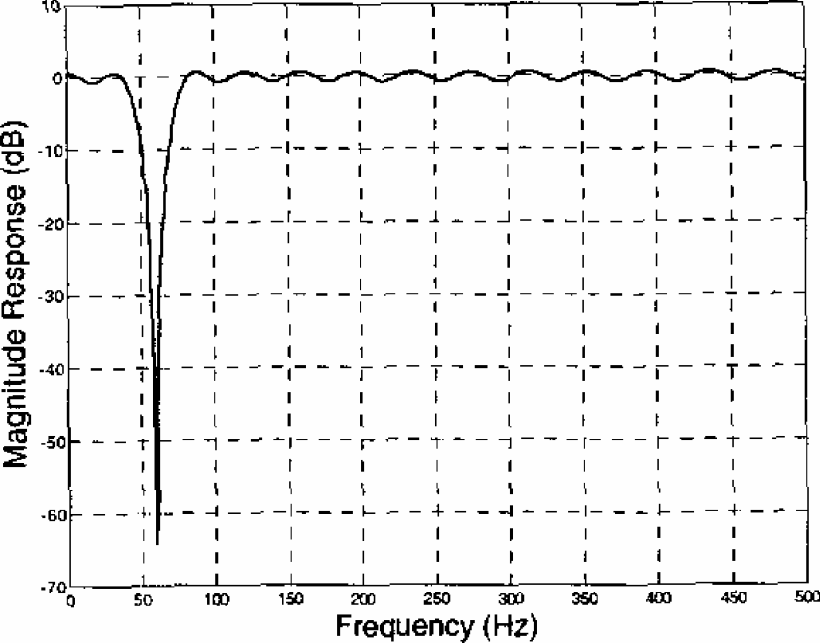
\includegraphics[scale=0.4]{figs/notch_fir_paper_2004.png}
		\caption{Result of notch filter FIR design using the Parks-McClellan algorithm. The filter order was 52.}
	\end{figure}
	\FloatBarrier
	 
\end{description}

\mbox{}\\
\noindent {\bf Problem 5: Hilbert transformer (25 points)}

In Homework \#4 you saw some applications of the Hilbert transform. In this problem, we will focus on the Hibert transformer, which is an LTI system used to calculate the Hilbert transform of time-domain signals. More specifically, the Hilbert transformer is used to phase-shift signals by 90 degrees. Hence, the output of a Hilbert transformer to a cosine is a sine of same frequency. This operation has applications in digital communication, radar systems, and medical imaging.

As discussed in class, the Hilbert transform is defined by the convolution:
\begin{equation}
	\mathcal{H}\{x(t)\} = \frac{1}{\pi t}\ast x(t) \Longleftrightarrow 	H_{HT}(j\Omega) = -j\mathrm{sign}(\Omega) = \begin{cases}
	-j, & \Omega > 0 \\
	0, & \Omega = 0  \\
	j, & \Omega < 0 \\
	\end{cases}
\end{equation}

We will approximate this by the following discrete-time frequency response
\begin{equation}
	H_{d}(e^{j\omega}) = -j\mathrm{sign}(\omega) = \begin{cases}
	-j, & 0 < \omega \leq \pi \\
	0, & \omega = 0  \\
	j, & -\pi < \omega < 0 \\
	\end{cases}
\end{equation}

Note that this filter acts as an all-pass filter (except at $\omega = 0$) with  90-degree phase shift. Its impulse response is given by
\begin{equation} \label{eq:hilbert-impulse}
	h_d[n] = \begin{cases}
	\displaystyle\frac{2}{\pi}\frac{\sin^2(\pi n/2)}{n}, &n \neq 0 \\
	0, & n = 0
	\end{cases}
\end{equation}

The impulse response has odd symmetry about $n = 0$ i.e., $h_d[n] = -h_d[-n]$. Hence, we can design linear-phase FIR systems to approximate $h_d[n]$.

For the questions below assume the filter order is $M = 30$ (i.e., 31 coefficients).

\noindent\textbf{Note:} Since the FIR filters you will design are linear phase, their frequency response will be approximately
\begin{equation}
	H(e^{j\omega}) \approx e^{-j\omega M/2}(-j\mathrm{sign}(\omega)) = \begin{cases}
	e^{-j(\omega M/2 + \pi/2)}, & 0 < \omega \leq \pi \\
	0, &\omega = 0 \\
	e^{-j(\omega M/2 - \pi/2)}, & -\pi < \omega < 0
	\end{cases} 
\end{equation}

Therefore, they'll look like an all-pass except around $\omega = 0$ and $\omega = \pi$, but they still have the property of phase shifting the input signal by 90 degrees. However, due to causality and the linear phase condition, the output signal will also be delayed by $M/2$ samples.

\begin{description}
	\item[(a)] \textbf{Window method}. Use the window method with the window of your choice to design a linear phase FIR filter $H_{win}(z)$ that will approximate $H_{d}(e^{j\omega})$. The impulse response of the Hilbert transformer in discrete time is given in \eqref{eq:hilbert-impulse}. Plot the magnitude and phase response of your design.
	
	\item[(b)] \textbf{Parks-McClellan}. Use the Parks-McClellan algorithm to design a linear phase FIR filter $H_{PM}(z)$ that will approximate $H_{d}(e^{j\omega})$. In your design, assume that the \underline{weight function} is 
	\begin{equation}
		W(\omega) = \begin{cases}
		0, & 0 \leq \omega < \Delta\omega \\
		1, & \Delta\omega \leq \omega \leq \pi-\Delta\omega \\
		0, & \pi-\Delta\omega < \omega \leq \pi
		\end{cases}
	\end{equation}
	where $\Delta\omega = 0.1\pi$. This means that your Hilbert transformer will only work between $0.1\pi$ and $0.9\pi$, since it will only have magnitude 1 in $[0.1\pi, 0.9\pi]$,  Naturally, you'd like to make $\Delta\omega$ as small as possible, but that will introduce undesired ripples in the passband. Feel free to try different values of $\Delta\omega$.
	
	Plot the magnitude and phase response of your design.

	\textit{Matlab hints:} 
	\begin{itemize}
		\item When using the function \texttt{firpm}, note that Matlab expects the filter magnitude $|H_{d}(e^{j\omega})|$ (parameter \texttt{a}). However, $|H_{d}(e^{j\omega})| = 1$ over all frequencies, except zero. To differentiate that from an all-pass filter, you have to pass the extra parameter \texttt{`hilbert'}: 
		\begin{equation*}
		\texttt{>> hpm = firpm(M, f, a, `hilbert');}
		\end{equation*}
		where \texttt{f} is the \underline{normalized} frequency vector and \texttt{a} is the magnitude at frequencies \texttt{f}. This way \texttt{hpm} will have odd symmetry.
		\item This question is already solved in the Matlab documentation of the function \texttt{firpm}.
	\end{itemize}
	
	\item[(c)] \textbf{Least-squares}. Use the least-squares algorithm (\texttt{firls}) to design a linear phase FIR filter $H_{ls}(z)$ that will approximate $H_{d}(e^{j\omega})$. Use the same assumptions and hints of part (b). Plot the magnitude and phase response of your design.
	
\end{description}

\mbox{}\\
\noindent {\bf Problem 6: Linear equalization (25 points)}

Figure~\ref{fig:linear_eq} shows the block diagram of a digital communication system. In this system, a sequence of bits $x[n]$ is transmitted over a channel, which is a causal LTI system with $z$-transform $C(z)$. Since the channel is causal its output depends not only on the present bit, but also on previous bits transmitted over the channel. Hence, the output of the channel is the result of interference of many bits. This phenomenon is called \textit{inter-symbol interference} (ISI). In addition to ISI, after the channel, a white and zero-mean Gaussian noise $r[n]$ with average power $\sigma^2 = 0.001$ is added to the signal. This models the noise from the receiver circuitry.

The filter $H(z)$ is an FIR linear equalizer, which should be designed to mitigate the interference introduced by the channel. 

\begin{figure}[h!]
	\centering
	\resizebox{0.7\textwidth}{!}{\begin{tikzpicture}[->, >=stealth, shorten >= 0pt, draw=black!50, node distance=2.5cm, font=\sffamily]
    \tikzstyle{node}=[circle,fill=black,minimum size=2pt,inner sep=0pt]
    \tikzstyle{block}=[draw=black,rectangle,fill=none,minimum size=1.5cm, inner sep=0pt]
    \tikzstyle{adder}=[draw=black,circle,fill=none,minimum size=1cm, inner sep=0pt]

	\node[node] (xc) {};
    \node[block, right of=xc] (Ch) {$C(z)$};
    \node[adder, right of=Ch] (add) {\Large $+$};
    \node[block, right of=add] (DSP) {$H(z)$};
	\coordinate[right of=DSP] (yc) {};
	\node[node, below of=add] (nw) {};
	
	%\coordinate (mid1) at ($(ADC.east)!0.5!(DSP.west)$) {};
	%\coordinate (mid2) at ($(DSP.east)!0.5!(DAC.west)$) {};
		
    \path (xc) edge (Ch);
    \path (Ch) edge (add);
    \path (add) edge (DSP);
    \path (DSP) edge (yc);
    \path (nw) edge (add);
    
    %\node[above = 0.5mm of mid1] {$x[n]$};
    %\node[above = 0.5mm of mid2] {$y[n]$};
    \node[above = 0mm of xc, text width = 1cm, align=center] {$x[n]$};
    \node[above = 0mm of yc, text width = 1cm, align=center] {$y[n]$}; 
    \node[right = 0mm of nw, text width = 3cm, align=center] {$r[n]\sim\mathcal{N}(0, \sigma^2)$}; 
    
    \node[below] at (Ch.south) {Channel};
    \node[below] at (DSP.south) {Linear equalizer};
\end{tikzpicture}}
	\caption{Diagram for linear equalization}
	\label{fig:linear_eq}
\end{figure}

For this problem, we will consider that the channel is the FIR filter given by
\begin{equation}
	C(z) = 0.4032 + 0.3992z^{-1}  + 0.1976z^{-2}
\end{equation}

When noise is not significant, the optimal linear equalizer is simply the inverse of the channel:
\begin{equation} \label{eq:zero-forcing}
	H(z) = C^{-1}(z) = \frac{1}{0.4032 + 0.3992z^{-1}  + 0.1976z^{-2}}
\end{equation}
which is an IIR filter. 

In the following questions you will design FIR filters to approximate $H(z)$. In all cases, assume that your FIR filter has order $M = 8$ (9 coefficients).
\begin{description}
	\item[(a)] \textbf{Window method}. Design an FIR filter to approximate $H(z)$ using the window method. Since $H(z)$ does not have discontinuities, you can use the rectangular window without problem. On the same graph, plot the frequency response of your FIR filter and $H(z)$. On a different graph, plot the \underline{unwrapped} phase response of your FIR filter and $H(z)$. Note that they are not linear phase.
	
	\textit{Hint:} use the Matlab function \texttt{impz} to obtain the impulse response of $H(z)$.
			
	\item[(b)] Test your linear equalizer using the function \texttt{simple\_channel.m}, available on Canvas. This function takes one parameter \texttt{h}, which is the coefficients of the FIR filter you designed. The function returns the bit-error rate (BER) (number of wrongly detected bits divided by total number of bits) of this system when the receiver equalizer has coefficients \texttt{h}. Hence, \texttt{simple\_channel(1)} returns the BER of the system without any equalization. Report the BER \underline{with} and \underline{without} equalization. For the given noise power, the BER of the equalized system should be close to 0. 
	\item[(c)] \textbf{Non-linear phase least-squares algorithm}. Now design an FIR filter using the least squares algorithm to approximate $H(z)$. Since $H(z)$ has no discontinuities, you can assume that the weight function is $W(\omega) = 1~\forall~\omega$. Moreover, since this filter should not be linear phase, you cannot use Matlab's \texttt{firls} function. Instead, use the least-squares algorithm as described in class. You may use the script \texttt{predicing\_bandlimited\_signals.m} as a starting point.
	
	On the same graph, plot the frequency response of your FIR filter and H(z). On a different graph, plot the \underline{unwrapped} phase response of your FIR filter and H(z).
	
	\textit{Note:} the filter you designed in this part should be (ideally) identical to the filter you designed in part (a), since the rectangular window minimizes the mean-square error (lecture notes 9, slide 33)
	
	\item[(d)] Estimate the noise power after the linear equalizer you designed.
	
	\textit{Note:} you should see that this value is much larger than $\sigma^2 = 0.001$. This happens because this equalizer tries to force ISI to zero at all costs, even if it enhances the noise. This type of equalizer is called \textit{zero-forcing linear equalizer}. A better choice of equalizer is called the \textit{minimum mean-square linear equalizer}, which tries to minimize ISI without excessively enhancing the noise.
	
\end{description}
\end{document}
